%!Mode:: "TeX:UTF-8"
%\begin{frame}
%    \frametitle{OUTLINE}
%    \begin{itemize}    
%        \item
%    \end{itemize}
%\end{frame}

\begin{frame}
    \begin{center}
        \LARGE \tt{GIT}
    \end{center}
\end{frame}

\begin{frame}
    \frametitle{Git基础}
    \begin{itemize}    
        \item 版本控制的概念
            \begin{description}
                \item[版本控制\footnote{\url{http://zh.wikipedia.org/wiki/\%E7\%89\%88\%E6\%9C\%AC\%E6\%8E\%A7\%E5\%88\%B6}}] 
                    是维护工程蓝图的标准作法,
                    能追踪工程蓝图从诞生一直到定案的过程。
                    此外,版本控制也是一种软件工程技巧,
                    借此能在软件开发的过程中,
                    确保由不同人所编辑的同一程式档案都得到同步。
            \end{description}
        \item 关于GIT
            \begin{description}
                \item[Git\footnote{\url{http://zh.wikipedia.org/wiki/Git}}] 
                    是一个由Linus Torvalds
                    为了更好地管理linux内核开发
                    而创立的分布式版本控制/软件配置管理软件。
            \end{description}
        \item 一个重要概念\footnote{\url{http://git-scm.com/book/en/Getting-Started-Git-Basics}}
            \begin{itemize}
                \item Git关心文件数据的整体是否发生变化。
                \item 其他版本管理系统则关心具体内容的差异。
            \end{itemize}
    \end{itemize}
\end{frame}

\begin{frame}
    \frametitle{git的版本控制模型}
    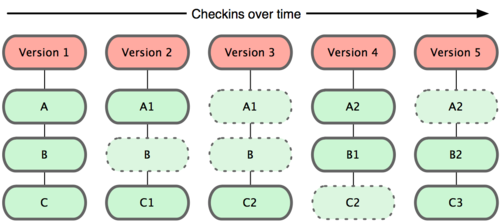
\includegraphics[width=10cm,keepaspectratio]{data/GitRevisionModel.png}
\end{frame}

\begin{frame}
    \frametitle{其他系统的版本控制模型}
    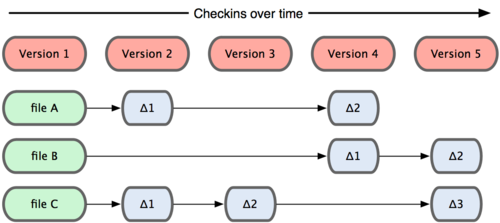
\includegraphics[width=10cm,keepaspectratio]{data/OtherRevisionModel.png}
\end{frame}

\begin{frame}
    \frametitle{分布式工作流程\footnote{\url{http://git-scm.com/book/en/Distributed-Git-Distributed-Workflows}}}
    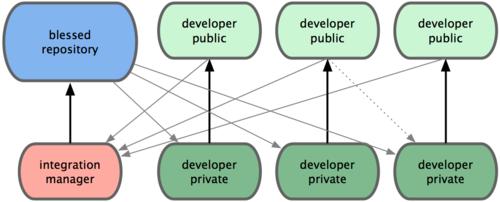
\includegraphics[width=10cm,keepaspectratio]{data/GitDistributedWorkflow.png}
    \begin{block}{我们的开发模式}
        \begin{itemize}
            \item 公共的仓库,由管理员负责
            \item 个人的仓库,由开发者自己管理
            \item 如果要将个人的代码合并如公共的仓库,
                  提交Pull Request,告诉管理员仓库的url和分支名。
        \end{itemize}
    \end{block}
\end{frame}

\begin{frame}
    \frametitle{Git的数据流}
    \begin{columns}
        \column{6.0cm}
            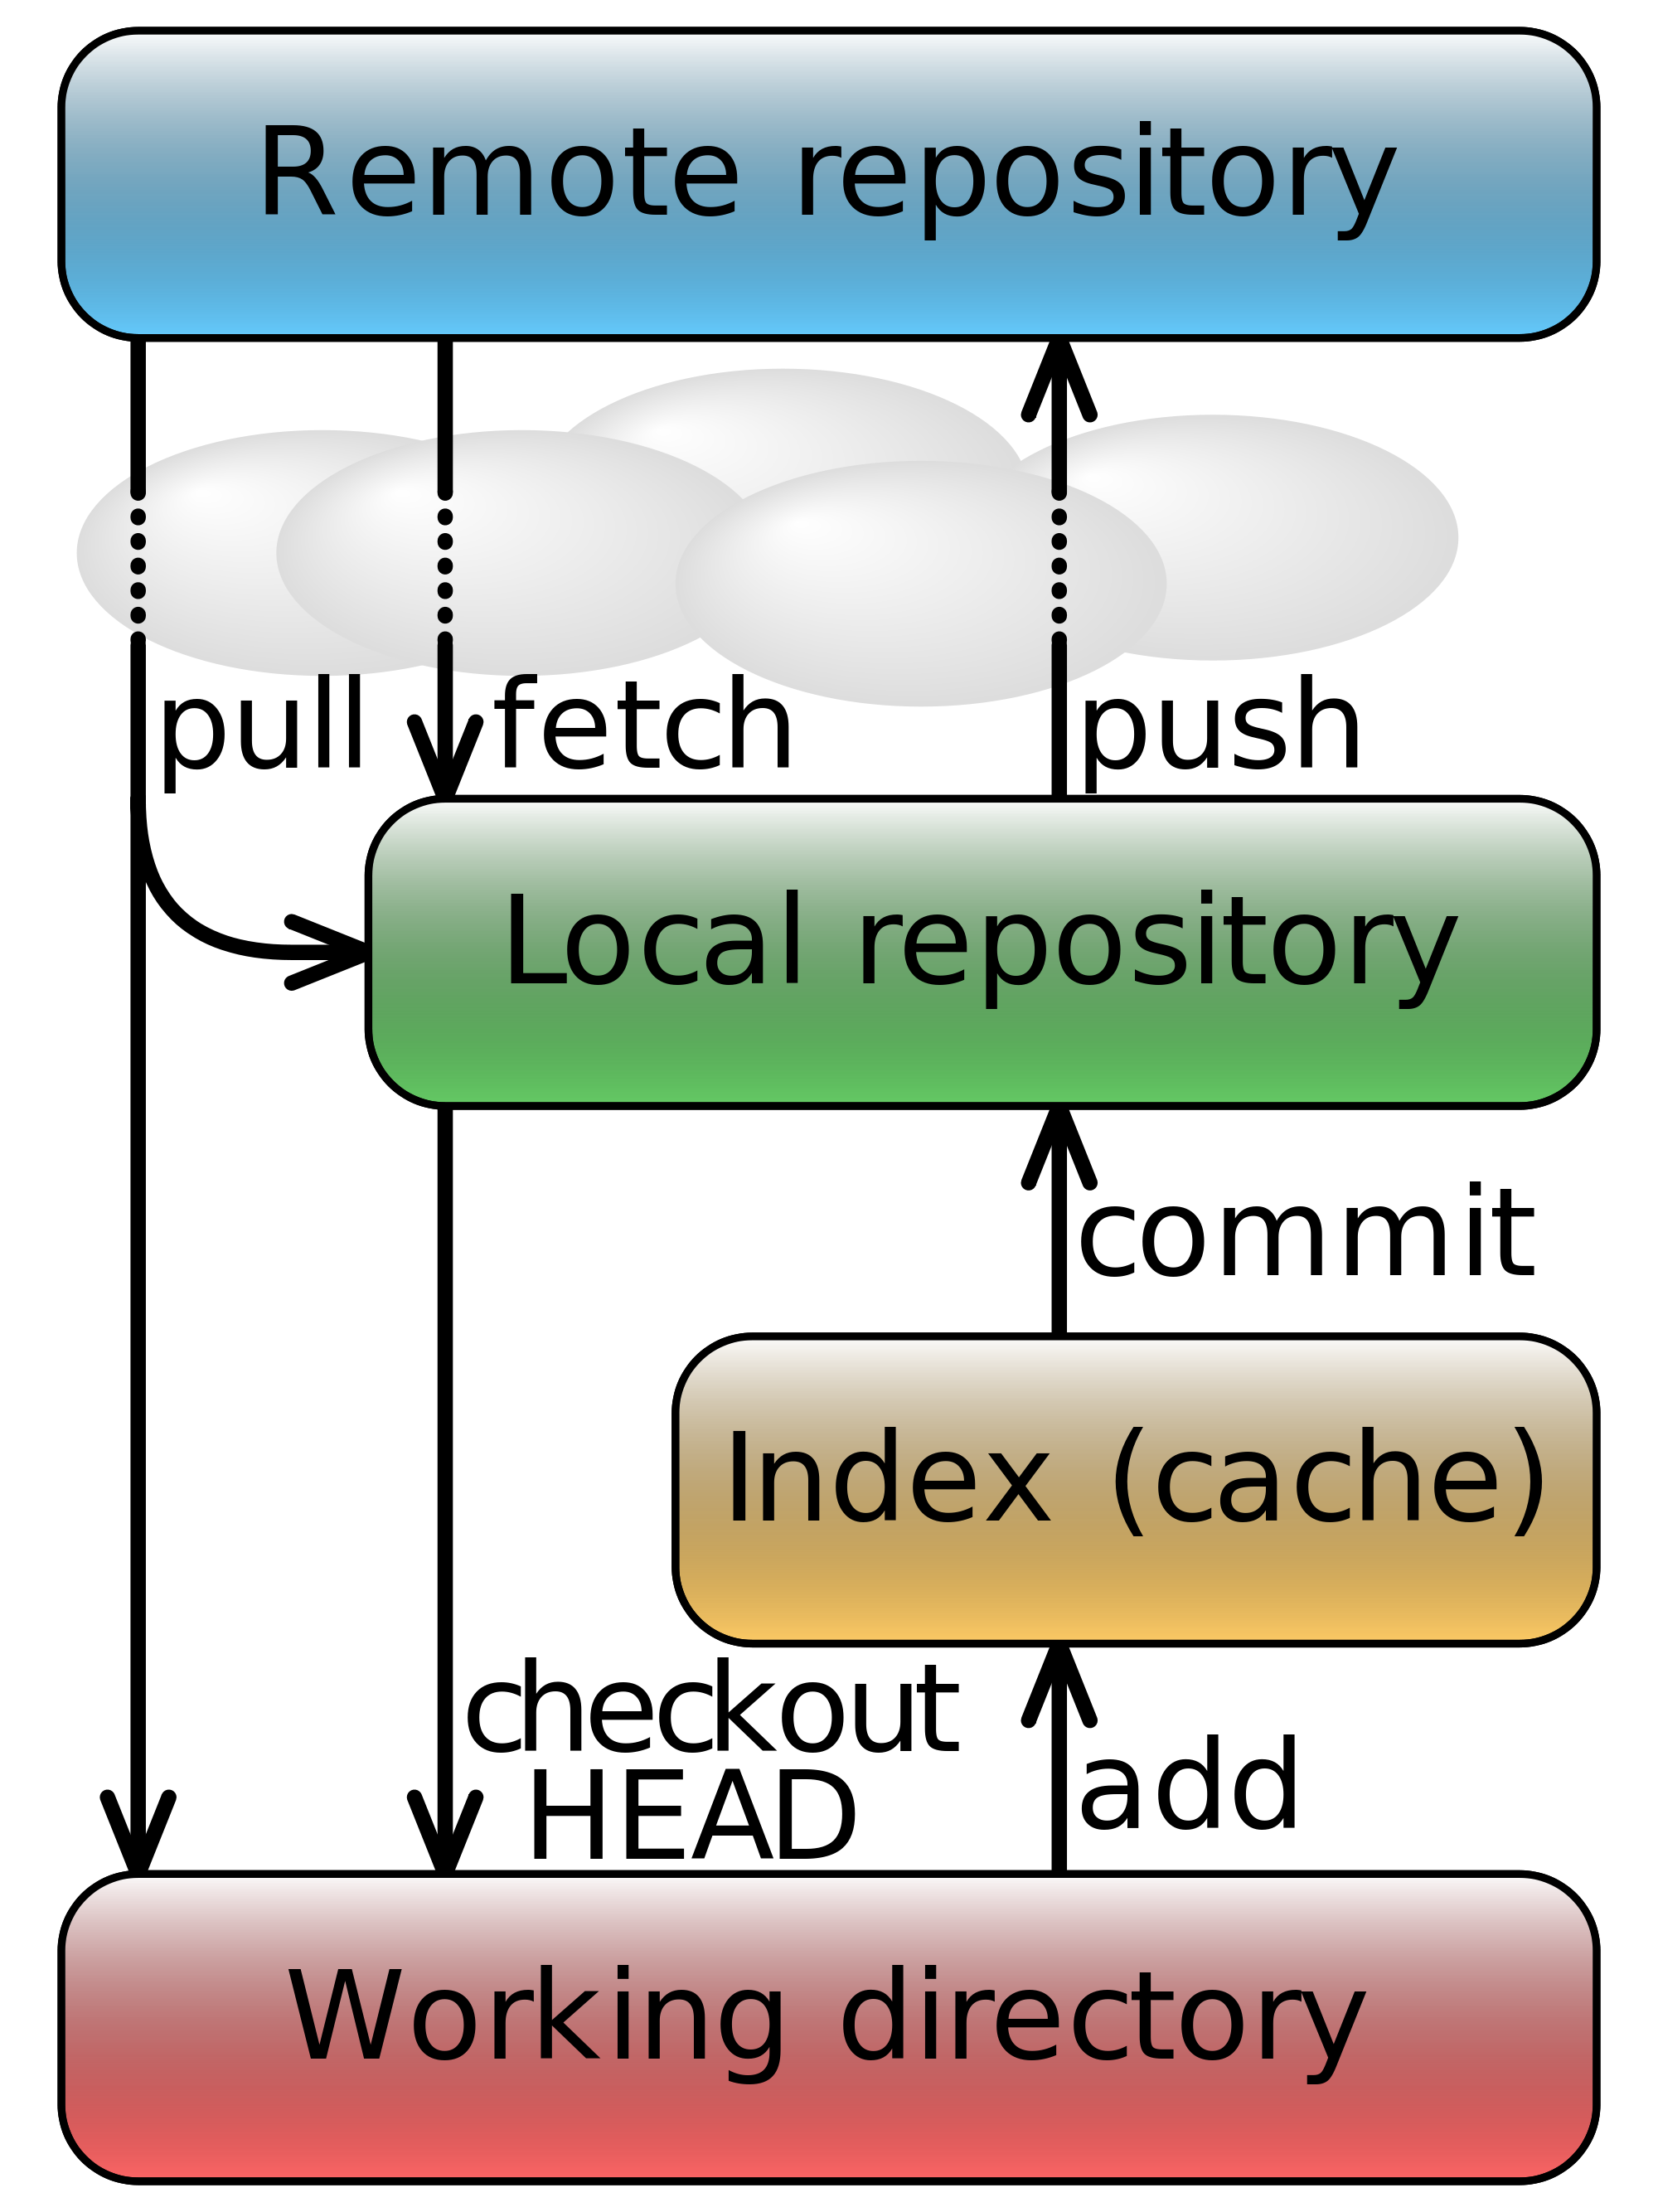
\includegraphics[height=8cm,keepaspectratio]{data/GitDataFlowSimplified.png}
            \label{pic:DataFlow}
        \column{4.5cm}
            \begin{itemize}
                \item 远程仓库
                \item 本地仓库
                \item 工作目录
            \end{itemize}
    \end{columns}
\end{frame}

